\documentclass[a4paper,12pt]{article}
\usepackage{graphicx}
\usepackage{float}
\usepackage{fancyhdr}
\usepackage{listings}
\lstset
{
  numbers=left,
  breaklines=true,
}
\pagestyle{fancy}
\rhead{Dane Johnson}
\title{CS-456 Project 3}
\author{Dane Johnson}
\date{April 18st, 2018}
\headheight=15pt
\begin{document}
\maketitle
\newpage
\section{Motivation}

This project was an attempt to demonstrate multiple ways of solving an NP-complete problem and to show to pros and cons
of each method as well as a way to demonstrate an example of an approximation algorithm and discuss when an approximation
would be useful and appropriate.

\section{Algorithms}
\subsection{Brute Force}
\subsubsection{Pseudocode}
\begin{lstlisting}[mathescape=true]
proc brute_force(G, s)
  for cycle in permute(G.V - {s})
    if len([s] + cycle + [s]) < min_cycle
      min_cycle $\gets$ [s] + cycle + [s]
  return min_cycle
proc permute(V)
  if len(V) == 1
    return V
  for u in V
    for permutation in permute(V - {u})
      permutations $\gets$ permutations + {permutation + {u}}
  return permutations
\end{lstlisting}
\subsubsection{Time Complexity}
This algorithm finds the shortest Hamiltonian Cycle by looking through every possible arrangement of nodes and determining which of them has the shortest distance. In order to accomplish this, the {\it permute} procedure creates all possible orderings of the nodes, an operation which takes $O(n!)$ time.
\subsubsection{Correctness Proof}
\begin{description}
\item [Invariant: ] After the $k$th iteration, $k$ cycles will have been considered for the shortest Hamiltion cycle, and the miniumum will be recorded.
\item [Initialization: ] $k$ is 0 initially, no paths have been considered and no shortest has been selected.
\item [Maintenence: ] After the $k$ iterations, the $k$th cycle is considered and, if it is the minimum yet considered, it is recorded.
\item [Termination: ] When the loop terminates, $k = n$, so all possible cycles have been considered and the minumum cycle has been recoreded.
\end{description}
\subsubsection{Empirical Validation}
\begin{figure}[H]
  \centering
  \textbf{Brute Force}\par\medskip
  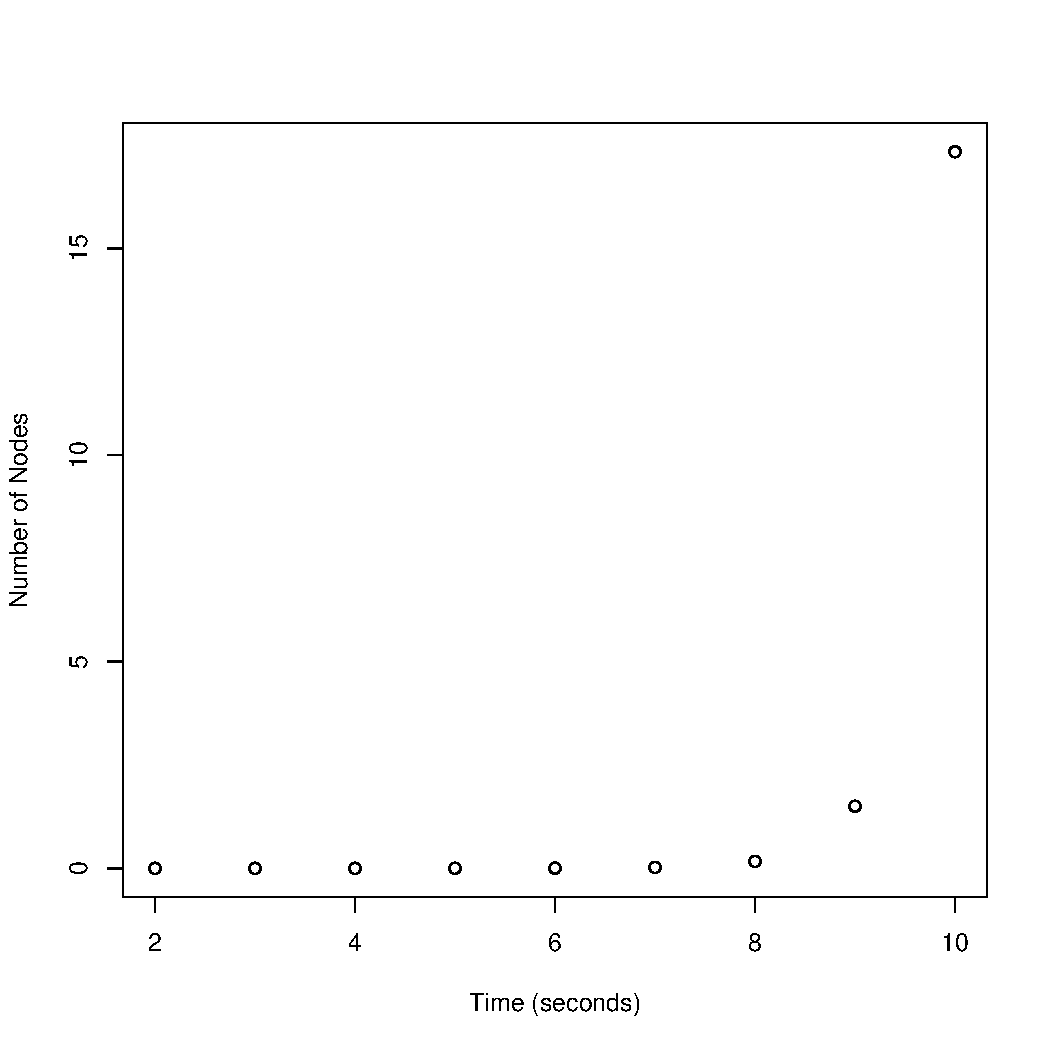
\includegraphics[width=1\linewidth]{BruteForce.pdf}
\end{figure}
Y axis in log scale.
\subsubsection{Observations}
Here we can see the data on a y-log graph. Even on a log graph, which would show polynomial relations as a straight line, we can still see a clear curvature. This would indicate that the time complexity of the algorithm is non-polynomial. Additionally, we can see that the algorithm begins to perform extremely poorly even at 10 nodes, taking a whole 17 seconds. 
\subsection{Branch and Bound}
\subsubsection{Pseudocode}
\begin{lstlisting}[mathescape=true]
proc branch-and-bound(G, s)
  state.placed $\gets$ {s}
  state.remaining $\gets$ G.V - {s}
  state.lower_bound $\gets$ lower_bound(state.placed, state.remaining)
  Q $\gets$ {state}
  while Q $\neq \emptyset$
    curr $\gets$ Q.extract_min()
    if curr is a solution
      if curr < solution
        solution $\gets$ curr
        prune Q for lower bounds < curr
    else
      Q $\gets$ Q + {next_states(curr)}
  return solution
proc next_states(state)
  next_states $\gets \emptyset$
  for $\forall u \in state.remaining$
    next_state.placed $\gets$ state.placed + {u}
    next_state.remaining $\gets$ state.remaining - {u}
    next_state.lower_bound $\gets$ lower_bound(next_state.placed, next_state.remaining)
    next_states = next_states + {next_state}
  return n
proc lower_bound(placed, remaining)
  add cost of all placed connections and cheapest edges from unplaced
\end{lstlisting}
\subsubsection{Time Complexity}
If the prune step is removed, this algorithm will generate the entire search tree, which will cause the algorithm to become a scan of the entire solution space. Given that, in the worst case, no pruning occurs, worrst case time complexity for the algorithm is still $O(n!)$.
\subsubsection{Correctnesss Proof}
\begin{description}
\item [Invariant: ] At the end of the $k$th loop, $k$ nodes of the search tree have been explored.
\item [Initialization: ] Initially, $k = 0$, and only the source node is on the tree 
\item [Maintenence: ] Each step, all children of the most promising node are added to the tree to be explored, and the $k$th most promising node has been explored
\item [Termination: ] After $n!$ iterations, $n!$ options have been explored and the search tree has been completely explored.
\end{description}
\begin{figure}[H]
  \centering
  \textbf{Branch and Bound}\par\medskip
  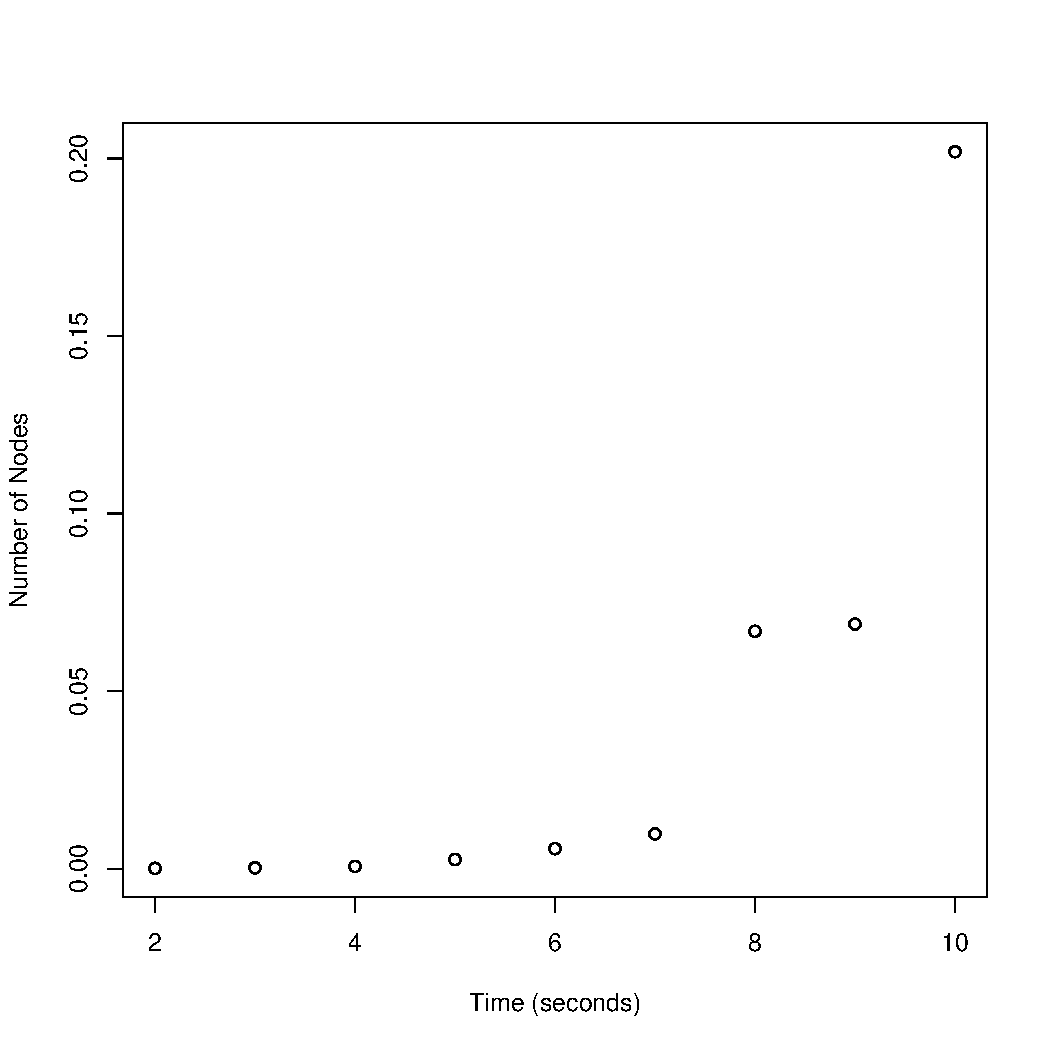
\includegraphics[width=1\linewidth]{BranchAndBound.pdf}
\end{figure}
Y axis in log scale.
\subsection{Observations}

\subsection{Dynamic Programming}
\subsubsection{Pseudocode}
\begin{lstlisting}[mathescape=true]
proc dynamic_programming(G, s)
  cost $\gets \emptyset$
  for i in G.V - {s}
    cost[{s, i}] = dist(s, i)
  for n - 2
    for i in G.V - {s}
     for $\forall$ n - 1 sized subsets
       
      
\end{lstlisting}
\subsubsection{Time complexity}
The time complexity of connecting a new node is $\Theta(|V|)$, Bellman-Ford is $O(VE)$, removing the node is $\Theta(|V|)$, and creating the new weight function is $O(E)$. From here, we are updating every row of the new matrix, which has height $V$, by running Dijkstra's algorithm on each node. The time complexity of Dijkstra is depenedent on the data strucure in use, which will be explored later, if a Min Priority Heap is used, it will be $O(VElg(V))$, and it will be $O(V^2lg(V))$ if a Fibonnacci Heap is used.
\subsubsection{Correctness Proof}
\begin{description}
\item [Invariant: ] The shortest path from a source vertex $u$ to any vertex $v$ can be found by running Dijkstras algorithm on the reweighted graph, and then recalculating based on the original weight
\item [Initialization: ] Initially, no sources have been selected, so the shortest path of all selected elements is found trivially.
\item [Maintenence: ] On each loop iteration, Dijkstra's algorithm finds the shortest path to the reweighted edge, and then the shortest path to each vertex is found by recalculating based on the original graph weight.
\item [Termination: ] When the loop terminates, Dijkstra's algorithm has been run on every vertex, finding the shortest path to all other vertices. Therefore all pairs shortest paths have been found.
\end{description}
\subsection{Min Priority Heap}
\subsubsection{Code Walkthrough}
The Min Priority heap is implemented simply as a binary heap that maintains the heap
property on inserts and extractions. Decreasing a key, an operation that is done for every edge in Dijkstra, can at maximum climb from the furthest leaf to the root, and thus takes$O(lg(n))$ time. Extracting a min, which is done for every vertex in Dijkstra, must restore the heap property when a node is removed, which at worst moves an item from the root to the furthest leaf, which takes $O(lg(n))$ time. Finally, insertions involve a key decrease, taking the same amount of time. In Dijkstra, this is done for every vertex. However, when used in Dijkstra, the operation that is done the more is the key decrease, which is performed for each edge. Therefore, the runtime of Dijkstra using a Min Heap is $O(Elg(V))$.
\subsubsection{Empirical Validation}
\begin{figure}[H]
  \centering
  \textbf{Sparse Graph}\par\medskip
\end{figure}
\begin{figure}[H]
  \centering
  \textbf{Dense Graph}\par\medskip
\end{figure}
\subsubsection{Observations}
Again the data is an average of 10 trials. Here we can clearly see the logarithmic relationship, as well as being able to see that the algorithm is much faster on sparse graphs than on dense graphs.
\subsection{Fibonacci Heap}
\subsubsection{Code Walkthrough}
The Fibonacci Heap uses a mergeable heap structure. It maintains the heap structure only on extractions. Decreasing a key in a Fibonacci Heap involves cutting a branch and inserting it into the root, which is an $\Theta(1)$ constant time operation. Extracting a min involves rebuilding the heap structure, which can be performed in $O(lg(n))$ time. Finally, insertions can be done in $\Theta(1)$ constant time as well, as it simply involves inserting into a root list. Since the decrease-key operation can be done in constant time, this speeds up Dijkstra's algorithm, as the key decreases are no longer the limiting factor. The time complexity for Dijkstra with a Fibonacci Heap now is limited by the number of vertices next to the explored area, reducing the runtime to $O(V^2lg(V))$.
\subsubsection{Empirical Validation}
\begin{figure}[H]
  \centering
  \textbf{Sparse Graph}\par\medskip
\end{figure}
\begin{figure}[H]
  \centering
  \textbf{Dense Graph}\par\medskip
\end{figure}
\subsubsection{Observations}
Again the data is an average of 10 trials. Here again the data are clearly logrithmic, although surprisingly Fibonacci Heap is still losing to a Min Heap. The overhead of the heap management still puts Fibonacci Heap performance below Min Heap, even when searching graphs of 400 vertices. Also we can see the algorithm is far more performant on sparse graphs.
\section{Conclusion}
An easily drawn conclusion is that Floyd-Warshall is a good choice only for dense graphs, as there is no optimization for sparse graphs. Min Priority heaps are generally a good choice, having a low barrier to entry to Fibonacci Heaps, as they are much easier to code and understand, while still allowing for the speedup from not running in cubic time. Fibonacci heaps are a good choice for major league processing, with maps with an extremely high number of vertices, but few edges. They are complex to implement, however, and in practice are slower than a Min Priority Heap on small inputs.
\end{document}
